\documentclass[a4paper,10pt,oneside]{article}
\usepackage[top=2cm,bottom=2cm,left=1cm,right=1cm]{geometry}
%\usepackage{fontspec}
\usepackage[utf8]{inputenc}
\usepackage{hyperref}
\usepackage{enumitem}
\usepackage{changepage}
\usepackage[table]{xcolor}
\usepackage{graphicx}
\usepackage{fancyhdr}
\pagestyle{fancy}
\usepackage{titlesec}
\usepackage{longtable}
\usepackage{setspace}
\usepackage{amsmath}
\usepackage{xcolor}
\usepackage{listings}

\hypersetup{
	colorlinks=true,      
	urlcolor=magenta,
	linkcolor  = black
}

\definecolor{mGreen}{rgb}{0,0.6,0}
\definecolor{mGray}{rgb}{0.5,0.5,0.5}
\definecolor{mPurple}{rgb}{0.58,0,0.82}
\definecolor{backgroundColour}{rgb}{0.95,0.95,0.92}

\lstdefinestyle{CStyle}{
	backgroundcolor=\color{backgroundColour},   
	commentstyle=\color{mGreen},
	keywordstyle=\color{magenta},
	numberstyle=\tiny\color{mGray},
	stringstyle=\color{mPurple},
	basicstyle=\footnotesize,
	breakatwhitespace=false,         
	breaklines=true,                 
	captionpos=b,                    
	keepspaces=true,                 
	numbers=left,                    
	numbersep=5pt,                  
	showspaces=false,                
	showstringspaces=false,
	showtabs=false,                  
	tabsize=2,
	language=C
}

\title{\Huge{\textbf{Tiva Based Daughter Board for Firebird V \\Software Manual}}}

\author{\textbf{ ERTS Lab IIT Bombay}}

\lhead{ }
\rhead{Manual for Tiva Based Daughter Board for Firebird V}
\lfoot{ERTS Lab IIT Bombay}

\renewcommand*\contentsname{\textbf{Table Of Content}}

\setcounter{secnumdepth}{4}

\titleformat{\paragraph}
{\normalfont\normalsize\bfseries}{\theparagraph}{1em}{}
\titlespacing*{\paragraph}
{0pt}{3.25ex plus 1ex minus .2ex}{1.5ex plus .2ex}

\begin{document}
	\large
	\maketitle
		
	\newpage
	\section{{\textbf{Credits}}}
	\textbf{\\\\ Version 1.0\\\date{\today}}% Right allign
	\\
	\\
	\\
	\\
	{\large{\textbf{Documentation Author(Alphabetical Order):}
			\begin{enumerate}
			\item Ayush Gaurav, Intern eYSIP 2017
			\item Nagesh K,  Intern eYSIP 2017
	\end{enumerate}
	\textbf{Credits(Alphabetical Order):}
		\begin{enumerate}
			\item Prof Kavi Arya, CSE IIT Bombay
			\item Nex Robotics Pvt. Ltd.
			\item Piyush Manavar, Team e-Yantra
			\item Saurav Shandilya, Team e-Yantra
	\end{enumerate}}
	\newpage
	\section{\textbf{Notice}}
	{\large The contents of this manual are subject to change without notice. All efforts have been made to
	ensure the accuracy of contents in this manual. However, should any errors be detected, e-yantra welcomes your corrections. You can send us your queries / suggestions at
	\href{mailto:helpdesk@eyantra.org}{Contact Us}\\}
	\newpage
	\doublespacing
	\tableofcontents
	\singlespacing
	\newpage 

		\newpage
		\section{Software Manual}
		
		
		\subsection{Programming the bot}
		The uC based board does not have an onboard programmer. So the JTAG pins tapped from a functional TIVA launchpad is connected to the JTAG headers present on the Daughter board. These connections are shown in the Figure1 and Figure2\\
		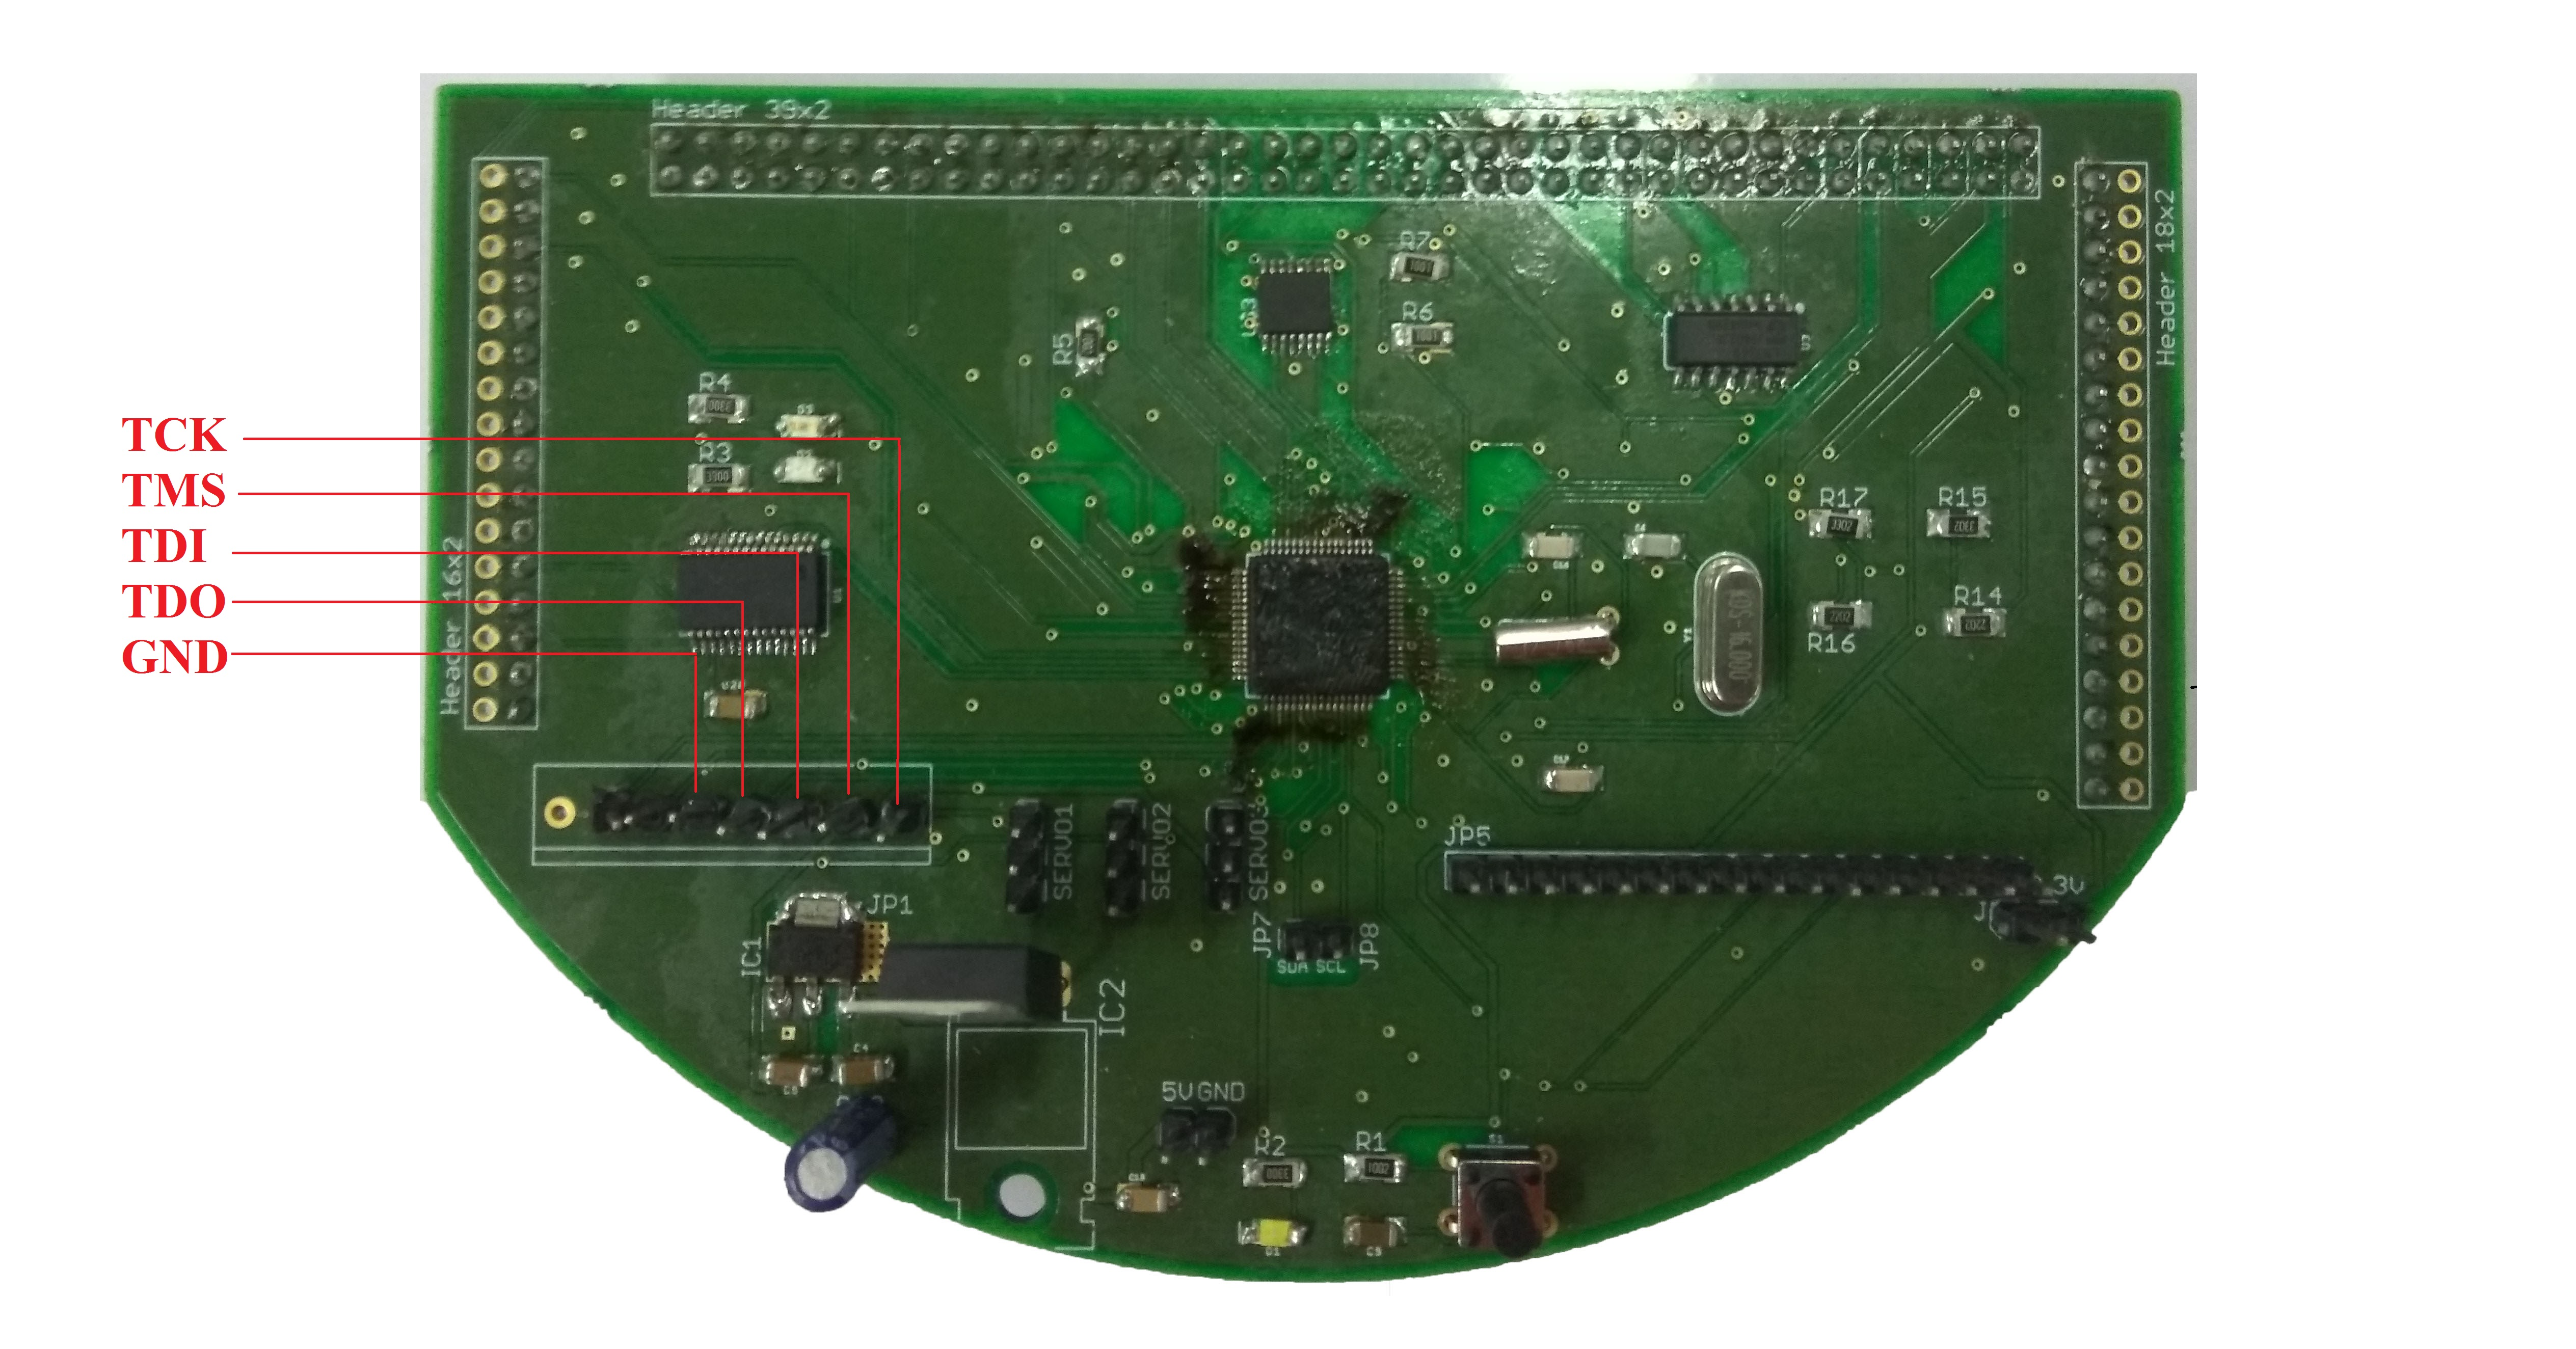
\includegraphics[width=10cm, height=6cm]{Pro}
		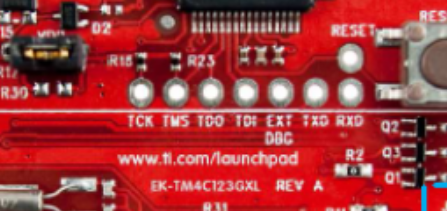
\includegraphics[width=6cm, height=4cm]{TI}\\
		
		\hspace{4cm}
		Figure1
		\hspace{6cm}
		Figure2\\
		{The TCK, TMS, TDI and TDO pins of the Daughter Board should be connected to the corresponding TCK, TMS, TDI and TDO pins of the TIVA launchpad.}			
			
			
		\subsection{\textbf{Simple I/O Operation}}
			{In this section, we will learn how to initialize GPIO pins in TM4C123G and use them for simple input-output operations. The code for TIVA is written in C99 programming standards with Hungarian standard for naming variables. }
			\subsubsection{\textbf{Header Files}}
				{Before writing the code we have to include certain header files to access the TivaWare API's. These header files are required for variable definition. The header files to included are given below. The purpose of each header file is explained in the following paragraphs.
				\begin{lstlisting}[style=CStyle]
					#include <stdint.h>
					#include <stdbool.h>
					#include "inc/hw_memmap.h"
					#include "inc/hw_types.h"
					#include "driverlib/sysctl.h" 
					#include "driverlib/gpio.h"				\end{lstlisting}
				\textbf{stdint.h: }This is used for defining variables according to C99 Standard.\\
				\textbf{stdbool.h: }This is used for defining variables according to C99 Standard.\\
				\textbf{hw\_memmap.h: }This contains the marcos defining the memory mapping of Tiva C Series devices. This includes base address locations of all the ports present in Tiva C Series devices. For example, the base address of port B can be accessed by "GPIO\_PORTB\_BASE". \\
				\textbf{hw\_types.h: }This header file includes macros for initialising a pin as input or output. For example, "GPIOPinTypeGPIOOutput" is used for defining a pin as an output pin. For example, "GPIOPinTypeGPIOOutput" is used for defining a pin as an output pin.  \\ 
				\textbf{sysctl.h :}This contains functions and macros for System Control API of DriverLib. \\
				\textbf{gpio.h: }This contains functions and macros for GPIO Control API of DriverLib. }
			\subsubsection{\textbf{Clock Setup}}
				{The TM4C123G contains 2  external clocks. The main oscillator contains a 16 MHz crystal and the Real Time Clock(RTC) contains a 32.768 MHz crystal. The TM4C123G can be configured to operate at different frequencies. In this case, we will configure the clock to operate at 40 MHz.}
				\begin{lstlisting}[style=CStyle]
					SysCtlClockSet(SYSCTL_SYSDIV_5|SYSCTL_USE_PLL|SYSCTL_XTAL_16MHZ|SYSCTL_OSC_MAIN); \end{lstlisting}
				{The 16MHz crystal drives the 400MHz PLL. There is default /2 divider in the path. We are further dividing this by 5, which means that the 400MHz PLL is divided by a total factor of 10. Hence the System Clock is set at 40MHz.\\
				Refer to the datasheet to configure the clock at different frequencies.} 	
			\subsubsection{\textbf{GPIO Configuration}}
				\begin{itemize}
				\item \textbf{Output} \\
				{The GPIO pins present in TM4C123G can be configured as input, output and interrupt. The clock of TM4C123G has to enabled for a port before using it as an input or output. This can be done by the following line of code.
				\begin{lstlisting}[style=CStyle]
					SysCtlPeripheralEnable(SYSCTL_PERIPH_GPIOB)  \end{lstlisting}
				In this case, clock is enabled for port B. After enabling the clock, we have to define the status of the pin. Consider an example where pin B6 should be defined as an output pin. This can be done by the following statement.
				\begin{lstlisting}[style=CStyle]
				GPIOPinTypeGPIOOutput(GPIO_PORTB_BASE, GPIO_PIN_6)  \end{lstlisting}
				
				Now, let us write a value into the pin B6 which is configured as an output pin. The following lines of code describe the same. In this code logic 1 is written to the pin.
				\begin{lstlisting}[style=CStyle]
				GPIOPinWrite(GPIO_PORTB_BASE, GPIO_PIN_6, 0x40) \end{lstlisting}
				\item \textbf{Input}	\\
				Now we define the same pin(B6) as an input pin. This can be done by the following statement. 
				\begin{lstlisting}[style=CStyle]
				GPIOPinTypeGPIOInput(GPIO_PORTB_BASE, GPIO_PIN_6)  \end{lstlisting}
				But this not sufficient to use it as an input pin. We have to enable the internal pull-up or pull-down resistor associated with a pin. This is shown below
								\begin{lstlisting}[style=CStyle]
				GPIOPadConfigSet(GPIO_PORTB_BASE,GPIO_PIN_6,GPIO_STRENGTH_2MA,GPIO_PIN_TYPE_STD_WPU)  \end{lstlisting}
				The internal pull-down resistor can be enabled by replacing WPU(Weak Pull Up) by WPD(Weak Pull Down).
				
				The code to read a value from a pin is given below. The value read has to be stored in a variable. In this case, the variable is test.  
				\begin{lstlisting}[style=CStyle]
					test=(GPIOPinRead(GPIO_PORTE_BASE, GPIO_PIN_6)\end{lstlisting}
				}
			\end{itemize}		
		\subsubsection{\textbf{Assignments}}
			\begin{itemize}
				\item The buzzer is connected to PF4 in Plug and Play board. Write a code to switch the buzzer on and off alternatively.
				\item The buzzer is connected to PA2 in uC based board. Write a code to switch the buzzer on and off alternatively.
				\item The motor connections are as shown below. Write a code to move the bot in forward, backward, left and right directions.
			\end{itemize}
		 	\begin{center}
					\begin{tabular}{|c|c|c|}
						\hline
						\textbf{Motor Pin} & \textbf{Pin Name(uC)} & \textbf{Pin Name(Plug and Play)}\\
						\hline
						L1 & PB0 & PF3 \\
						\hline
						L2 & PB1 & PB3 \\
						\hline
						PWM Left & PF3 & PF2 \\
						\hline
						R1 & PF4 & PC4 \\
						\hline
						R2 & PA5 & PC6 \\
						\hline
						PWM Right & PA6 & PC5\\
						\hline
					\end{tabular}
		 	\end{center}
\end{document}